\documentclass[a4paper,10pt]{article}
\usepackage[french]{babel}
\usepackage[utf8]{inputenc}
\usepackage[left=2.5cm,top=2cm,right=2.5cm,nohead,nofoot]{geometry}
\usepackage{url}
\usepackage{graphicx}
\usepackage{float}
\usepackage[colorinlistoftodos]{todonotes}
\usepackage{hyperref}

\linespread{1.1}



\begin{document}

\begin{titlepage}
\begin{center}
\textbf{\textsc{UNIVERSIT\'E LIBRE DE MONTR\'EAL}}\\
%\textbf{\textsc{Faculté des Sciences}}\\
%\textbf{\textsc{Département d'Informatique}}
\vfill{}\vfill{}
\begin{center}{\Huge Rapport : TP1 - Sudoku}\end{center}{\Huge \par}
\begin{center}{\large Pierre Gérard, Alexandre Savard}\end{center}{\Huge \par}
\vfill{}\vfill{} \vfill{}
\begin{flushleft}{\large \textbf{IFT 3335 Intelligence artificielle: Introduction}}\hfill{Jian-Yun Nie, William Lechelle}\end{flushleft}{\large\par}
\vfill{}\vfill{}\enlargethispage{3cm}
\textbf{Année académique 2015~-~2016}
\end{center}
\end{titlepage}

%\begin{abstract}
%Ce rapport présente ...
%\end{abstract}


\tableofcontents

\pagebreak


\section{Formulation du problème}

% Alex

\section{Search}

% Alex

\section{Hill-climbing}

% Pierre
\subsection{Implémentation}
L'algorithme a été implémentée de manière à ce que la grille initiale soit remplie de manière totalement aléatoire. L'état initiale est donc cette grille initiale. On peut le visualiser comme la racine d'un arbre. Il a 9 enfants. Chaque enfant correspond a la permutation de (case1,case2) dans un des carré de dimension 3x3 telle que cette permutation minimise le nombre de conflit global. la permutation optimale est trouvé en les testant toutes à l'intérieur d'un carré 3x3

% condition d'arrêt

Cela permet d'affirmer que la probabilité que l'algorithme trouve une solution optimale tend vers 1 pour un très grand nombre d'essaie avec des configurations initiales différentes.

\subsection{Résultat}

Ci dessous un exemple de l'exécution du Hill-Climbing.
\begin{verbatim}
 --- INPUT ---
. . 3 |. 2 . |6 . . |
9 . . |3 . 5 |. . 1 |
. . 1 |8 . 6 |4 . . |
---------------------
. . 8 |1 . 2 |9 . . |
7 . . |. . . |. . 8 |
. . 6 |. . 8 |2 . . |
---------------------
. . 2 |. . 9 |5 . . |
8 . . |2 . 3 |. . 9 |
. . 5 |. 1 . |3 . . |
---------------------

Hill climbing
4 8 3 |9 2 1 |6 7 5 |
9 6 7 |3 4 5 |8 2 1 |
2 5 1 |8 7 6 |4 9 3 |
---------------------
5 4 8 |1 6 2 |9 3 7 |
7 2 9 |5 3 4 |1 6 8 |
3 1 6 |7 9 8 |2 5 4 |
---------------------
1 3 2 |6 8 9 |5 4 6 |
8 7 4 |2 5 3 |7 1 9 |
6 9 5 |4 1 7 |3 8 2 |
---------------------
ECHEC, malgre 20 test de configuration initiale differente
Ci dessus, un maximum local (4 conflits restant)
\end{verbatim}
Comme indiqué, il reste 4 conflits et la solution proposé n'est pas une solution valide de sudoku, mais s'en approche.
Pour des grilles plus simple l'algorithme trouve bien la solution comme on peut voir ci-dessous.
\begin{verbatim}
	 --- INPUT ---
. . . |9 2 . |. 5 7 |
9 . 7 |. 4 5 |8 2 1 |
2 5 1 |8 7 6 |4 9 3 |
---------------------
5 4 8 |1 . 2 |9 7 6 |
7 2 9 |5 6 4 |1 3 8 |
1 3 . |7 9 8 |2 4 5 |
---------------------
3 7 2 |6 8 9 |5 1 4 |
8 1 4 |2 5 3 |7 6 9 |
. 9 5 |4 1 7 |3 8 2 |
---------------------

Hill climbing
4 8 3 |9 2 1 |6 5 7 |
9 6 7 |3 4 5 |8 2 1 |
2 5 1 |8 7 6 |4 9 3 |
---------------------
5 4 8 |1 3 2 |9 7 6 |
7 2 9 |5 6 4 |1 3 8 |
1 3 6 |7 9 8 |2 4 5 |
---------------------
3 7 2 |6 8 9 |5 1 4 |
8 1 4 |2 5 3 |7 6 9 |
6 9 5 |4 1 7 |3 8 2 |
---------------------

Succes !
\end{verbatim}
Pour cette grille simple, Hill climbing a bien trouvé la solution optimale.
\subsection{Analyse des résultats}
Il n'est pas surprenant que Hill Climbing, un algorithme de recherche local, ne trouve pas de solution optimale. En effet, il est basé sur des changement locales et trouve régulièrement de bonne solution mais rarement la solution optimal. La figure suivante illustre cela.
\begin{figure}[H]
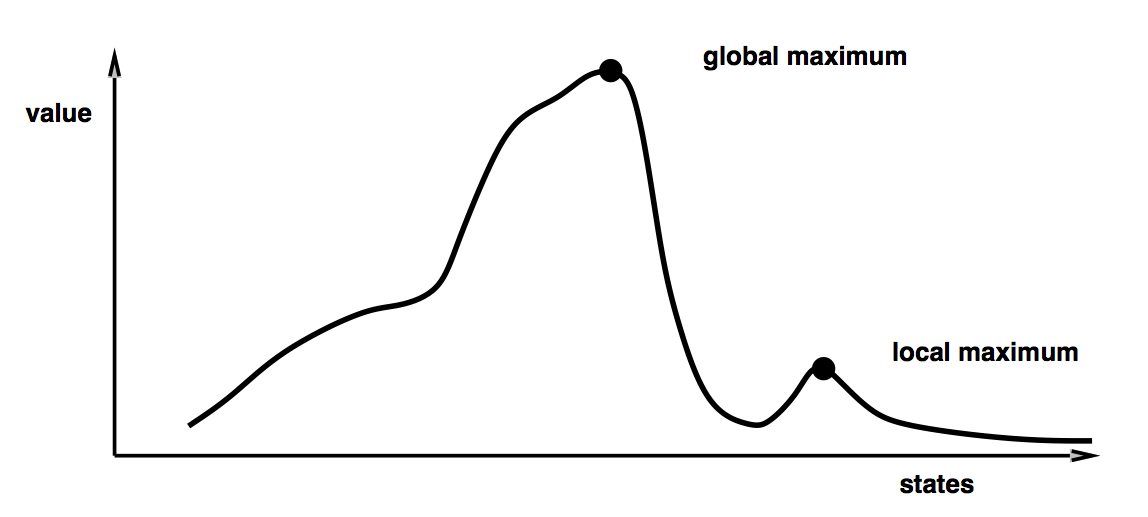
\includegraphics[scale=0.25]{images/hill-climbing.png}
\centering
\caption{Representation du maximum local}
\end{figure}
Une fois au maximum local, notre algorithme s'arrête comme il n'a pas de meilleur voisin. Il est incapable de dire si il existe un meilleur sommet.

Une meilleur technique serait le Simulated annealing, non demandé ici. 
\section{Heuristic search}

\subsection{Implémentation}
\subsection{Résultat}
\subsection{Analyse des résultats}

% Pierre

\section{Comparaison}

% Alex


\section{Heuristique bonus}


\end{document}
